\documentclass[12pt]{article}

%
% Packages
%

\usepackage{etoolbox}
\usepackage[capposition=top]{floatrow}
\usepackage{graphicx}
%\usepackage{caption}
%\usepackage{subcaption}
\usepackage{placeins}
\usepackage{setspace}
\usepackage{array}
\usepackage{fullpage}
%\usepackage[margin=1.5in]{geometry}
\usepackage{hyperref}
\usepackage{natbib}
\usepackage{microtype}
\usepackage{rotating}
\usepackage{amsmath}
\usepackage{morefloats}
\usepackage{float}
\usepackage{caption}
\usepackage{xcolor}
\usepackage[T1]{fontenc}
\usepackage[utf8]{inputenc}
\usepackage{authblk}
\usepackage{lmodern}

\hypersetup{
    colorlinks,
    linkcolor={black},
    citecolor={black},
    urlcolor={blue}
}
\usepackage{color,colortbl}
\usepackage{geometry}

\newcommand{\red}{\color{red}}
\newcommand{\blue}{\color{blue}}
\newtoggle{final}
%\togglefalse{final}
\toggletrue{final}


%
% Some utilities
%
%\usepackage{todonotes} % doesn't work - tikz lib too old
% define a mc=margincomment command
\iftoggle{final}{
   \newcommand{\mc}[2]{#1} % make margincomments go away
   \newcommand{\tc}[2]{#1} % make text comments go away
}%else
{
   \newcommand{\mc}[2]{% 1 referenced text 2 initials 3 comment
       \textcolor{blue}{#1}
       \marginpar{\scriptsize\textbf\raggedright\textcolor{red}{#2}}}
  \newcommand{\tc}[2]{\textcolor{blue}{#1}[\textcolor{red}{#2}]}
}

%
% Layout
%
\iftoggle{final}{
  \geometry{left=1.0in,right=1.0in,top=1.0in,bottom=1.0in}
}%else
{
  \geometry{left=0.5in,right=2.0in,top=1.0in,bottom=1.0in,marginparwidth=1.5in}
  }


\begin{document}

%Lane Adjustment Ahead: Uncertainty in Commuting Zones, Causes and Impacts
\title{Recalculating ... : How Uncertainty in Local Labor Market Definitions Affects Empirical Findings\thanks{The analysis, conclusions, and opinions expressed herein are those of the author(s) alone and do not necessarily represent the views of the U.S. Census Bureau or the Federal Deposit Insurance Corporation. All results have been reviewed to ensure that no confidential information is disclosed, and no confidential data was used in this paper. This document is released to inform interested parties of ongoing research and to encourage discussion of work in progress. Much of the work developing this paper occured while Mark Kutzbach was an employee of the U.S. Census Bureau.}}
\author[1]{Andrew Foote}
\author[2]{Mark J. Kutzbach}
\author[1,3]{Lars Vilhuber}
\affil[1]{Center for Economic Studies, U.S. Census Bureau}
\affil[2]{Federal Deposit Insurance Corporation}
\affil[3]{Labor Dynamics Institute, Cornell University}
\maketitle

\begin{center}
\textbf{[Preliminary Draft - Do not cite without authors' permission]}
\end{center}

\begin{abstract}

This paper evaluates the use of commuting zones as a local labor market definition. We revisit Tolbert and Sizer (1996) and demonstrate the sensitivity of definitions to two features of the methodology. We show how these features impact empirical estimates using a well-known application of commuting zones. We conclude with advice to researchers using commuting zones on how to demonstrate the robustness of empirical findings to uncertainty in definitions.
\end{abstract}


\doublespacing

%%%%%%%%%%%%%%%%%%%%%%%%%%%%%%%%%%%%%%%%%%%
\section{Introduction \label{sec:intro}}
Local labor markets are an important unit of analysis in labor economics, both in the theoretical and empirical literatures. Theoretical papers emphasize characteristics of a local labor market including common wage and rent levels \citep{Roback1982,Moretti2011}, as well as job-finding and unemployment rates \citep{HL2012,SS2014}.

In empirical labor economics, researchers may be interested in estimating the effect of some local, exogenous shock on labor market outcomes, and an important decision in any research design is defining the area that is directly affected by the shock. In estimating this effect, researchers have a number of different definitions of local labor markets from which to choose. \citet{BK1992}, \citet{Wozniak2010}, and \citet{KW2011} use the state, while other researchers use metropolitan areas \citep{BH2000,Card2001,Notowidigdo2011,Diamond2016}, while still others use counties \citep{MRR2015,FGS2015}.

One alternative labor market definition is commuting zones, which were originally defined by \citet{TS1996} (henceforth, TS1996). Commuting zones have two distinct advantages over the above definitions. First, they span the entire United States, allowing researchers to measure effects for the entire country rather than just metropolitan areas. Second, commuting zones group together counties based on commuting flows, which implies some level of economic integration (metropolitan areas are also based on commuting flows). The definition acknowledges that labor markets are not constrained by county and state lines, but are based on relevant linkages between counties.

Given these advantages, commuting zones have been used in a number of influential papers in the labor economics literature, including \citet{ADH2013}, as well as \citet{Yagan2016}, \citet{Restrepo2015} and \citet{AM2015}. Despite their widespread use, to the best of our knowledge, the methodology underlying commuting zone definitions and its impact on empirical estimates has not received much scrutiny. 

Our paper makes three contributions to the literature on local labor markets. First, we outline a number of methodological issues that researchers should be aware of when they use the commuting zone definitions. Second, we show how these methodological issues impact empirical estimates. Our findings suggest that researchers should consider evaluating the sensitivity of results to local labor market definitions. We propose two main ways that researchers can test to see if their results are robust to the uncertainty induced by commuting zones. Finally, we propose an alternative method similar to the one employed by Tolbert and Sizer, which allows us to measure integration beyond just commuting flows. We define a metric for the quality of a regionalization definition, and show that our proposed method performs better than alternative methods.

The remainder of the paper proceeds as follows. We describe the data we use in Section \ref{sec:data}, and then in Section \ref{sec:definitions} describes the commuting zone definition and methodology in detail. In Section \ref{sec:issues}, we discuss a number of issues with the commuting zone methodology. In Section \ref{sec:adhreplication}, we demonstrate how these issues impact empirical estimates. Finally, in Sections \ref{sec:objfn} and \ref{sec:ourmeth}, we discuss our measure of local labor market integration and methodology for defining local labor markets. Section \ref{sec:conclusion} summarizes and discusses next steps. 




%%%%%%%%%%%%%%%%%%%%%%%%%%%%%%%%%%%%%%%%%%%
\section{Commuting Zone Data and Methodology \label{sec:method}}
As an alternative to metropolitan statistical areas (or Core Based Statistical Areas), many researchers use
Commuting Zones because they cover the entire country and group counties based on commuting flows, which is a
measure of labor market integration. However, few researchers are familiar with the methodology used to develop
these zones. To that end, this section describes the methodology used by Tolbert and Sizer (1996) in
developing the zones.\footnote{The methodology was originally used in Tolbert and Killian (1987), but the 1996
paper is much more widely cited, and the zones from that paper are the ones most commonly used.}

The Economic Research Service (ERS), an agency under the U.S. Department of Agriculture for which this
methodology was developed, distributes commuting zone definitions on its website. Commuting Zones are
especially relevant for the economic analysis of rural areas because they include all counties, not just urban
counties.

The methodology used by TS1996 has two important components: the dissimilarity matrix, which measures how ``far'' observations are from one another, and the clustering method, which decides how observations are divided into groups. The next two subsections outline how TS1996 address these two components.

\subsection{Dissimilarity Matrix}

The dissimilarity matrix (or conversely, similarity matrix) is a representation of the relative distance between pairs of counties, as measured by an entry in the matrix $D_{ij}$.\footnote{The clustering method used dictates using a dissimilarity or similarity matrix; one is just the complement of the other.} TS calculated the dissimilarity matrix $D$, where an entry $D_{ij}$ is the dissimilarity of county $i$ from county $j$, as below:

\begin{equation}\label{eqn:diss}
D_{ij} = 1- \frac{f_{ij}+f_{ji}}{min(rlf_{i},rlf_j)}
\end{equation}

In the above equation, $f_{ij}$ is the number of commuters who live in county $i$ and work in county $j$, and $rlf_i = \sum_j f_{ij}$ (including $f_{ii}$) is the measure of the resident labor force. TS1996 use the 1990 Journey-to-Work data, which tabulates the commuting information from the 1990 Census Long-form response.\footnote{Other releases of commuting zones have used 1980 and 2000 data. All three are available at \url{http://www.ers.usda.gov/data-products/commuting-zones-and-labor-market-areas.aspx}.}

\subsection{Clustering Method}

After constructing this dissimilarity matrix, TS1996 use it as an input into their clustering method. In general, clustering methods are used in data science to decide which observations are similar to one another, usually by dividing the observations into distinct groups. In their application, TS1996 use the average-linkage hierarchical clustering algorithm (PROC CLUSTER in SAS). The hierarchical clustering method uses the dissimilarity matrix in the following way. To begin, every county is its own cluster. Then, it finds the lowest value $D_{ij}$ in the dissimilarity matrix, and combines those two counties together. It then recalculates the dissimilarity values between the new cluster and all other clusters in the following way:\footnote{There are multiple distance measures that one can use for a clustering procedure; this is the measure used by TS1996.}

\begin{equation}
D_{KL} = \frac{1}{N_K N_L} \sum_{i \in C_k} \sum_{j \in C_L} D_{ij}
\end{equation}

Where $K$ and $L$ are clusters, and $D_{ij}$ is calculated as in Equation \ref{eqn:diss}.

This process continues until the researcher stops the process by choosing a ``cutoff'' height, $H$, such that if $D_{KL}>H$, then $K$ and $L$ do not merge.

We illustrate this process in Appendix Figure \ref{fig:caliclusters}, which shows the hierarchical progression of how counties are clustered together for California. In the top left-hand corner, only a few counties have joined at a height of $H=0.8$. As we increase the height from 0.8 to 0.88, more counties are joined together, which is also true when the height is 0.96. Finally, at a height of 1, almost all the counties have merged together, forming one large cluster and a few much smaller clusters.

\subsection{Our Replication}
\FloatBarrier

In order to replicate the clustering result in TS1996, which we  refer to as FKV1990, we use the 1990 Census JTW data and the methodology described above, with one important exception. Because of computing power constraints in 1996, TS1996 divided the country into six overlapping regions and performed the clustering algorithm on each region separately, and then manually resolved conflicts in overlapping regions. This decision has two consequences for users: first, the height cutoffs across regions are not the same, because there is a normalization step before the algorithm merges observations. Second, it induces some subjectivity, since there are likely conflicts in cluster assignment in areas with overlapping regions.

Rather than follow their methodology and divide the country into regions, we run the hierarchical clustering algorithm on the entire country, and use the height cutoff that most closely replicates their original zones, which we find to be 0.9418. TS1996's zones and our replication are in Figure \ref{fig:czreplication}, and our summary statistics comparing the zones are in Table \ref{tab:replication}.

While our replication does not perfectly match their zones, this is not surprising, because we did not split the country into overlapping regions. With that caveat, our replication matches the moments from the commuting zones closely, and for a given county, about 80\% of the counties in our new zones match with the counties in the original zones.
\begin{figure}[tbh]\centering
\begin{tabular}{cc}
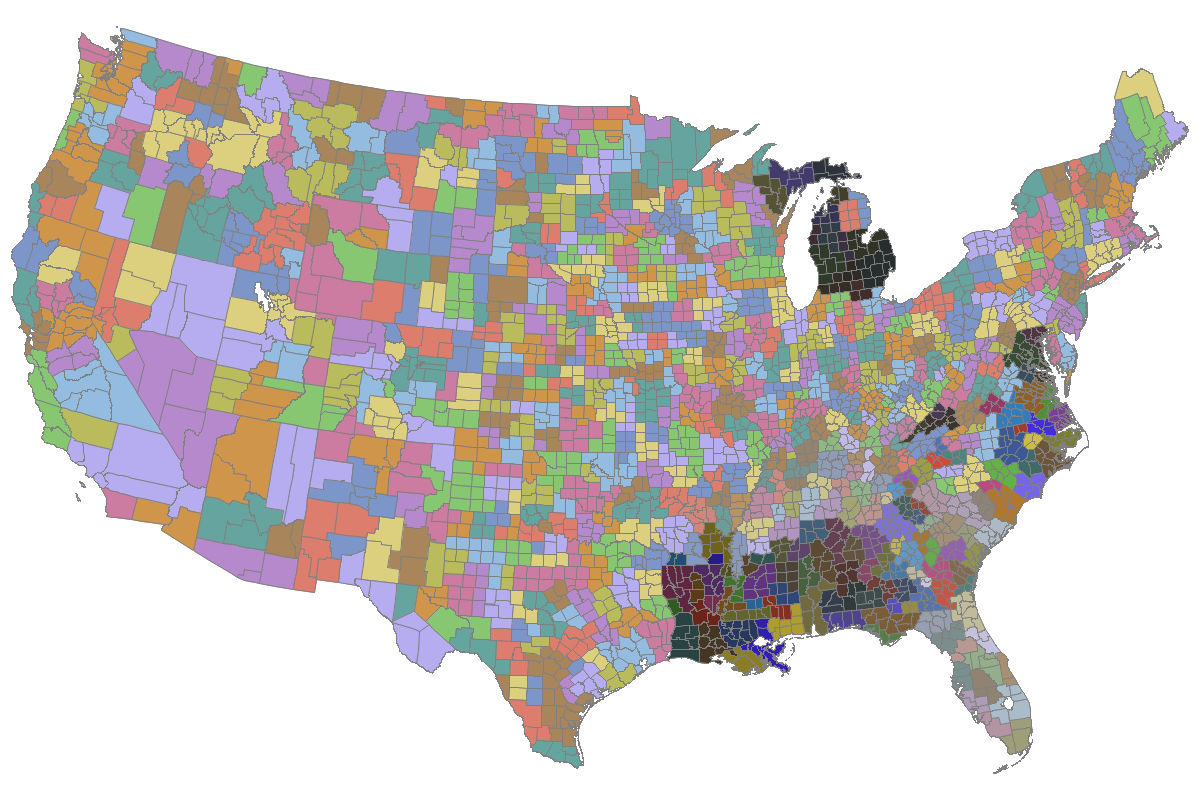
\includegraphics[scale=0.25]{./figures/commutingzones.png}&
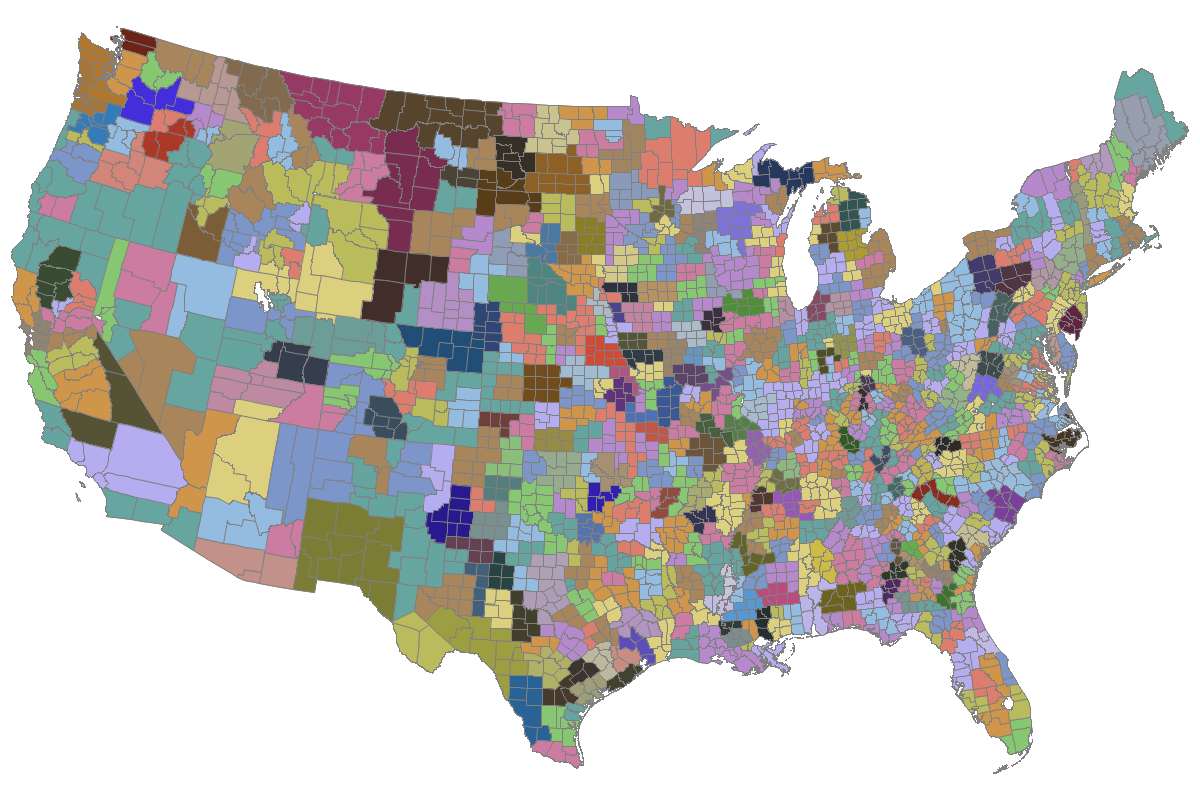
\includegraphics[scale=0.25]{./figures/clustermap_jtw1990_x.png}\\
Commuting Zones from TS1996 & Replication of Commuting Zones \\
\end{tabular}
\caption{Replication of Commuting Zones from TS1996: County Mapping \label{fig:czreplication}}
\end{figure}

% source: name of SAS program
% Last updated:

\begin{table}\centering
\caption{Replication of Commuting Zones from TS1996: Summary Statistics \label{tab:replication}}
\begin{tabular}{lcc}
\hline\hline
       & TS1990 &  FKV1990  \\
       \hline
Mean Cluster Size &  4.24  & 4.19 \\
Median Cluster Size & 4 & 4 \\
Number of Clusters & 741 & 741  \\
Number of Singletons & 62 &  10 \\
\hline
\multicolumn{3}{p{4in}}{\footnotesize \textit{Notes}: Both TS1990 and FKV1990 are based on JTW tabulations from the 1990 Census. Summary statistics for TS1990 are from Table 8 of TS1996.}\\
\end{tabular}
\end{table}


%Mark will look at writing a more efficient macro for this


%%%%%%%%%%%%%%%%%%%%%%%%%%%%%%%%%%%%%%%%%%%
\section{Design Sensitivity \label{sec:dsens}}
While commuting zones are used by researchers as a convenient measure of local labor markets, they have a number of shortcomings for empirical research that are not regularly discussed in the literature. In this section, we evaluate the sensitivity of commuting zone definitions, focusing on two aspects of the TS1996 methodology. First, we show that if there is uncertainty in the input data, the resulting commuting zone definitions can vary substantially. Second, the resulting clusters are sensitive to the decision of when to stop merging clusters, which implies that small changes in the chosen cutoff height can affect the number and size of the clusters. Overall, this uncertainty and subjectivity in the commuting zone definitions contributes to conventional standard errors understating the true level of uncertainty in the estimates, which we show when we return to this issue with our empirical replication in the next section.

\subsection{Sensitivity of Clustering Results to Underlying Error}

Given the reliance of TS1996 on the commuting flows data, we want to analyze the extent to which the outputs of the TS1996 methodology are sensitive to errors in this data. First, recall equation \ref{eqn:diss} for the entries of the dissimilarity matrix. If $f_{ij}$ is measured without error, then the distance between counties $i$ and $j$ is also measured without error. However, if the flows are measured with error, $\epsilon_{ij}$, then we actually have an estimate of $D_{ij}$, which is $\hat{D}_{ij}$, which can be expressed as below (assuming without loss of generality that $rlf_i < rlf_j$):


\begin{align*}
\hat{D}_{ij} &= 1 - \frac{f_{ij} + \epsilon_{ij} + f_{ji} + \epsilon_{ji}}{\hat{rlf}_i} \\
&= 1- \frac{f_{ij} + f_{ji}}{rlf_{ij} + \sum_j \epsilon_{ij}} +  \frac{\epsilon_{ij} + \epsilon_{ji}}{rlf_{ij} + \sum_j \epsilon_{ij}}
\end{align*}

We assume that $E[\epsilon_{ij}]=0$ and that $\epsilon_{ij} \perp \epsilon_{ik} \forall k$. However, even if $E[\epsilon_{ij}]=0$, that does not imply that $E[\hat{D}_{ij}] = D_{ij}$. Furthermore, we cannot rely on the limit properties of the error distribution, because we only have one realization of the commuting flow, which is calculated from survey responses. Additionally, we know that $\frac{\epsilon_{ij}}{f_{ij}}$ is larger for small flows. This will increase $D_{ij}$ for some small counties and decrease it for others. Because of the hierarchical nature of the clustering method, this error will affect the formation of all other clusters in the data.\footnote{Additionally, because heights are normalized in the procedure, it also affects where the effective cutoff is, even for counties unaffected by errors in flows.}

To demonstrate how this measurement error affects the outcome of the clustering procedure, we use the published margins of error (MOE) from the 2009-2013 ACS Journey to Work data to calculate the ratio $MOE_{ij}/f_{ij}$ for different sized flows.\footnote{These flow size bins are the following percentile bins: 0-50; 50-90; 90-95; 95-99; and 99+.} We project these ratios onto the flow bins from the 1990 Journey to Work data (which does not publish margins of error), to have an estimated MOE.\footnote{There are other possible projections of the margins of error from one dataset to another. The Census Long form is designed to be a one-in-six sample for one year, while the ACS 5-year summary is designed to 5 years with a one-in-fifty sample each year. The smaller sample size typically results in higher margins of error in the ACS for comparable statistics. The uncertainty implied be our implementation may be thought of as an upper bound.} Using these estimated MOEs, we then obtain different realizations of the commuting zones in the following way:

\begin{enumerate}
	\item For each origin-destination pair ($i,j$), we draw $\epsilon_{ij}$ from a normal distribution with mean 0 and standard deviation $MOE_{ij}/(2 \times 1.64)$, since the MOE is the 90\% confidence interval.
	\item Calculate the new flow value, $\hat{f_{ij}} = f_{ij} + \epsilon_{ij}$, with negative values set to zero.
	\item Re-calculate each dissimilarity matrix entry $\hat{D}_{ij}$. 
	\item Re-run the hierarchical clustering procedure, using the same cutoff as the replication.
	\item Store the new clusters, and calculate the following statistics: average number of counties in a cluster; number of clusters; and total number of counties in a different cluster than the one they were originally assigned.
\end{enumerate}

We iterate over this procedure 1000 times in order to obtain distributions for these statistics. These graphs are shown in Figure \ref{fig:sensitivity}, where the red vertical dashed lines are the values that would be obtained using only the published figures. The figures show that the average cluster size varies considerably from the result the published figures would yield. Additionally, the share of the population that is mismatched is on average about 5\% of the US population, a small but non-negligible number. Overall, the underlying measurement error in the data causes uncertainty in the cluster definitions, which is exacerbated by the sharp cutoff imposed in cluster analysis.

\begin{figure}
\caption{Sensitivity Analysis \label{fig:sensitivity}}
\begin{tabular}{ccc}
%\includegraphics[scale=.5]{../figures/numclusters_jtw1990.png}& 
%\includegraphics[scale=.5]{../figures/mean_clussize_jtw1990.png}&
%\includegraphics[scale=.5]{../figures/mismatchedcounties_jtw1990.png} \\ 
(a) Number of clusters & (b) Average Number of Counties & (c) Mismatched Counties \\
\end{tabular}
\end{figure}

\subsection{Choosing Cluster Height}

Another sensitive feature of the methodology used by TS1996 is choosing the cutoff value above which no clusters can form. \cite{TK1987} describe the algorithm for choosing a cutoff value as follows (see page 15): ``As a rule of thumb, a normalized average distance of 0.98 was considered sufficient distance between sets of counties to treat them as separate [Labor Market Areas].'' The article does not provide an analysis of the sensitivity to changing the cutoff marginally up or down. \cite{TS1996}, in an effort to minimize methodological differences between commuting zones for 1980 and 1990, use the same cutoff with no further evaluation for the 1990 data. In this subsection, we investigate how sensitive the resulting clusters are to the choice of the cutoff value.

\begin{figure}
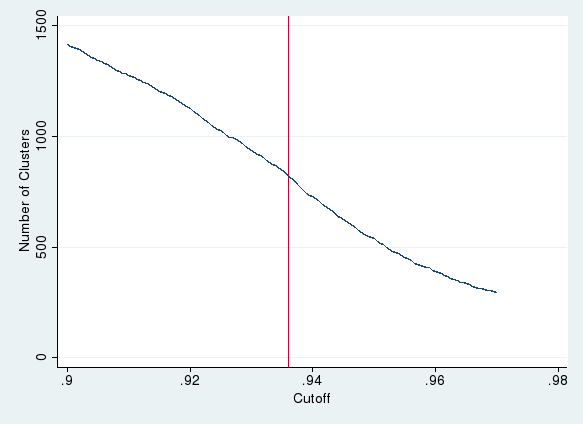
\includegraphics[scale=0.5]{./figures/numclus_cutoff.png}
\caption{Effect of Cluster Height on Number of Clusters \label{fig:cutoff_count}}
\emph{Note:} Authors' calculations using methodology outlined in Section \ref{sec:method}.
\end{figure}

Figure \ref{fig:cutoff_count} shows the number of clusters that form at various height cutoffs using the national 1990 JTW data, with the vertical line indicating the cutoff value we chose to replicate TS1990 (0.9418). The key takeaway from this figure is that it is theoretically ambiguous where a researcher should choose to stop merging clusters. Additionally, increasing or decreasing the cutoff has implications for the number of resulting clusters. Increasing it to 0.9428 decreases the number of clusters by 19, while using a cutoff of 0.9408 cause the number of clusters to increase by 17.

As we described above, the measurement error in commuting flows causes some uncertainty in terms of the true dissimilarity matrix, and hence the true cluster heights. Because of the presence of a strict cutoff, some clusters that would have formed if $D_{ij}$ were measured without error do not form, and vis-versa. More broadly, TS1996 provide no empirical guidance for choosing the optimal cutoff and cluster size other than referring to expert knowledge. While outside the scope of the current paper, future work may explore data-driven methods to determine whether there is an optimal number of clusters for certain uses.


%%%%%%%%%%%%%%%%%%%%%%%%%%%%%%%%%%%%%%%%%%%
\section{Empirical Sensitivity \label{sec:esens}}
In the previous section, we showed that there are a number of margins on which clustering methodologies
are sensitive, both in terms of the uncertainty in the input data as well as the choice of the number of
clusters. However, these issues are only important for empirical labor economists to the extent that these
sensitivities impact empirical estimates in a meaningful way. To that end, in this section, we demonstrate
the consequences of these sensitivities using a well-known paper that uses commuting zones.

\citet{ADH2013} estimate the impact that increased trade competition from China had on manufacturing
employment in the United States. To estimate this effect empirically, they use variation in the initial
distribution of manufacturing employment at the commuting zone level, and national increases in imports
from China by manufacturing subsector. Because Autor et al. use commuting zones as their definition of
local labor markets, their empirical analysis may be impacted by the issues outlined above.\footnote{We
want to acknowledge that the authors have been incredibly helpful in the process of replicating their
paper, both in providing data and helping to troubleshoot, and were receptive to this exercise.}

Their main estimating equation in the paper is as follows:

\begin{equation}\label{eqn:adh}
\Delta L_{it}^m = \gamma_t + \beta_1 \Delta IPW_{uit} + \beta_2 X_{it} + e_{it}
\end{equation}

Where $\Delta L_{it}^m$ is the decadal change in manufacturing employment in Commuting Zone $i$ following year $t$, $\Delta IPW_{uit}$ is the import exposure measure for the United States, and $X_{it}$ are control variables. All regressions are weighted by population share of the commuting zone.

\subsection{Replication of ADH}

Since we use slightly different methods of aggregating data, we compare the main estimates from \citet{ADH2013} (Table 1 in their paper) to our replication, which we show in Table \ref{tab:adhreplication}. Each cell in the table is a coefficient from a different regression, and for simplicity we just estimate it for the time period 1990-2000 (other results available upon request). The first column shows the estimates from their paper, while the second column changes the import exposure measures to our replicated measure. In the third column, we use our estimate of the change in manufacturing employment amd weights, rather than the estimate and weights from their data. The final column clusters on commuting zone rather than state.

% source: name of SAS program
% Last updated:

\begin{table}\centering
\caption{China Syndrome Replication and Comparison, 1990-2000 \label{tab:adhreplication}}
\begin{tabular}{lcccc}
\hline\hline
       & ADH Estimate & Our RHS & Our LHS and Weight & CZ Clustering  \\
       \hline
$\Delta IPW_{cz,t}$ & -0.8875 & -0.8871 & -0.8748 & -0.8748 \\
                   & (0.1812) & (0.1811) & (0.1527) & (0.1243) \\

\hline
\multicolumn{5}{p{6in}}{\footnotesize \textit{Notes}: Table from author's calculations, using data from \citet{ADH2013} and constructed data, based on equation \ref{eqn:adh}. Column 1 is Table 2, Column 1 from ADH (2013). Column 2 replaces their measure of import exposure to ours. Column 3 replaces their measure of change in manufacturing employment and CZ-specific weights with ours. Column 4 does not cluster on state. Standard errors are in parentheses. All coefficients are significant with p-values less than 0.01.}\\
\end{tabular}
\end{table}



Overall, the estimates are considerably stable, giving us confidence that we are properly replicating their initial findings. We now turn to demonstrating how these estimates are affected by the concerns with the commuting zone definitions themselves.

\subsection{Sensitivity to Errors in Flows Data}

First, we show how the estimate is affected based on MOE in the commuting flows input data. For this exercise, we use the 1000 realizations of the commuting zones that we generated in the previous section.

\begin{figure}\centering
\caption{Distribution of Effect, 1990-2000 \label{fig:1990dist}}
\begin{tabular}{c}
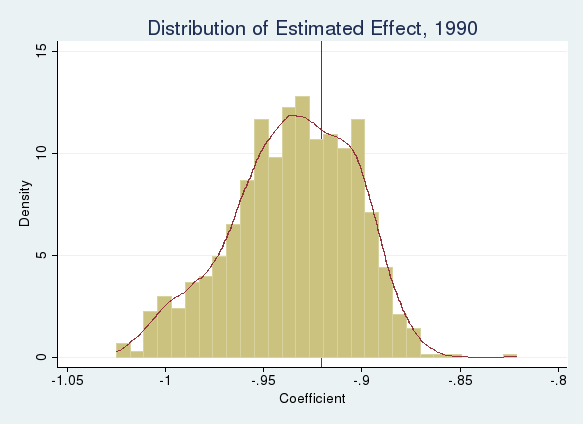
\includegraphics[scale=.3]{./figures/1990_distribution.png}\\
\multicolumn{1}{p{4.5in}}{\footnotesize \emph{Note:} Histogram plots estimates of $\beta_1$ from equation \ref{eqn:adh}, based on commuting zone realizations as outlined in Section \ref{sec:issues}.}
\end{tabular}
\end{figure}

[need a graph of t-statistics]

Using these different commuting zone definitions, we re-estimate Equation \ref{eqn:adh}. The coefficients from this exercise are graphed in Figure \ref{fig:adh_estimates}, which shows the distribution of the estimated effect for the 1990-2000 period. The red vertical line shows the estimate using the published flows data from our national replication of TS1996. The estimates are somewhat dispersed, with the left tail of the distribution almost 10\% lower than the estimate from ADH; however, the values are within two standard errors of the original estimate. Additionally, the distribution is skewed to the right.

Another way to summarize the results of this exercise is to look at the distribution of T-statistics, which is the pivotal statistic, and comparing that statistic with the critical values.

[say more about this here]

This exercise demonstrates that there is additional uncertainty induced by the construction of the commuting zones that is not addressed in empirical estimates that use these definitions, which may overstate the precision of the results.

\subsection{Sensitivity to Chosen Cutoff}

In addition to the uncertainty that is induced by underlying errors in the commuting flows, in Section 4.2 we showed that the decision of where to stop the clustering process was rather arbitrary, since there is no clear guidance on what cutoff is most appropriate. To demonstrate how the cutoff choice affects estimates of $\beta_1$ from Equation \ref{eqn:adh}, we generate clusteres based on cutoffs between 0.9 and 0.97 and estimate the equation using the resulting clusters.

\begin{figure}\centering
\caption{Differences in Effect Based on Cluster Cutoff \label{fig:cutoff_dist}}
\begin{tabular}{cc}

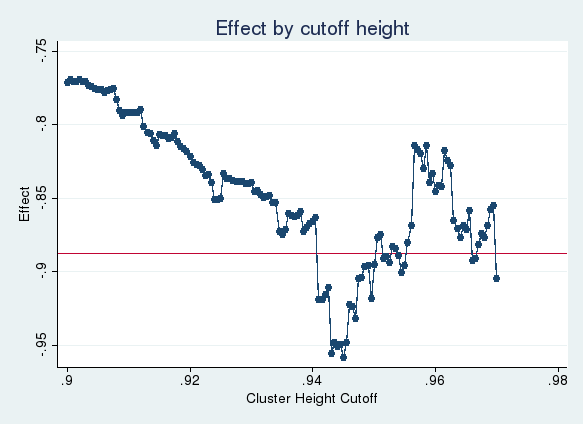
\includegraphics[scale=.35]{./figures/cutoff_1990.png} & 
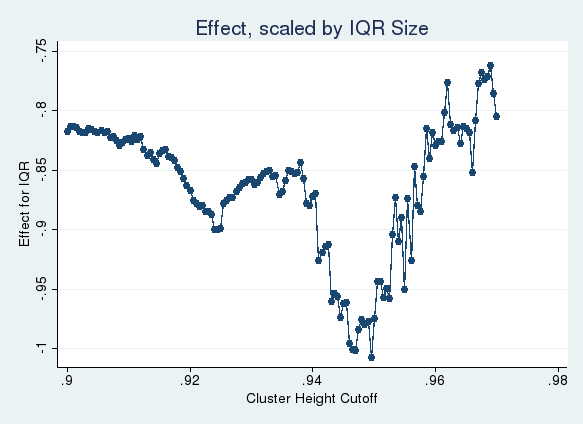
\includegraphics[scale=.35]{./figures/cutoff_iqr_1990.png}\\
(a) Effect by Cutoff Height & (b) Effect by Cutoff Height, Scaled by IQR \\
\multicolumn{2}{p{6.5in}}{\footnotesize \emph{Note:} Author's calculations based on replication of Tolbert and Sizer's method. Panel (a) shows estimates of $\beta_1$ from equation \ref{eqn:adh} for different definitions of commuting zones based on height cutoff, while Panel (b) shows estimates of $\beta_1$ scaled by the difference in exposure between the 25th and 75th percentile commuting zone. The horizontal line in panel (a) is the main estimate from \citet{ADH2013}}
\end{tabular}
\end{figure}

Figure \ref{fig:cutoff_dist} displays the results of this exercise, where panel (a) shows the raw coefficient and panel (b) shows the coefficient scaled by the interquartile range of $\Delta IPW_{uit}$, since that changes depending on the number of clusters. In panel (a),  the red horizontal line is the estimate from ADH.

Again, our results show that there is some variation in the estimate based on the cutoff value. Around the cutoff value that most closely replicates TS1996, the estimate is the most negative. However, cutoff values marginally higher or lower give different results, because the number of clusters changes quickly at that point. Given the sensitivity of estimates to the chosen cutoff, best practices for a researcher would be to report estimates for a broad range of possible cutoffs.	

\subsection{Advice to Researchers}

From the results above, it is clear that current commuting zone definitions overstate the uncertainty of zone assignment, which has implications for empirical results. Importantly, this uncertainty manifests itself on two different margins: uncertainty about zone assignment due to errors in the flows, and uncertainty about zone assignment due to the chosen cutoff. 

Given this uncertainty, we have two pieces of advice for researchers using commuting zones. First, we suggest using all realizations of commuting zones, to incorporate the additional uncertainty because of the flow errors. Second, we suggest displaying results for a variety of different cutoff values. To aid researchers in this effort, we provide datasets and code online [insert url] that include a crosswalk from county to all the realizations of commuting zones, as well as commuting zones for different cutoff values.





%%%%%%%%%%%%%%%%%%%%%%%%%%%%%%%%%%%%%%%%%%%
\section{Conclusion \label{sec:conclusion}}
Recent influential papers in labor economics have used commuting zones as an alternative definition to local labor markets. However, no one has carefully analyzed the methodology used to construct commuting zones and how it may impact empirical findings. Our paper contributes to this literature by analyzing this methodology and its implications for empirical applications.

We document that the commuting zone methodology is sensitive to uncertainty in the input data and parameter choices and we demonstrate how these features affect the resulting labor market definitions. Furthermore, we demonstrate that uncertainty in local labor market definitions also affects empirical estimates that use commuting zones as a unit of analysis. In future work, we want to explore other clustering methods, which are less history-dependent, as they may come to more globally optimal solutions. We also want to develop a measure with which to compare candidate zones against one another, using multiple metrics of local labor market integration.



%%%%%%%%%%%%%%%
% BIBLIOGRAPHY
%%%%%%%%%%%%%%%
\clearpage
\singlespacing

\bibliographystyle{aea}
\bibliography{bibliography}

\newpage
\appendix
\section*{Tables and Figures Appendix}
\FloatBarrier

\appendix
\setcounter{table}{0}
\renewcommand{\thetable}{A\arabic{table}}   
\setcounter{figure}{0}
\renewcommand{\thefigure}{A\arabic{figure}}   

\begin{figure}[th]
\caption{Various Height Cutoffs for California \label{fig:caliclusters}}
\begin{tabular}{cc}
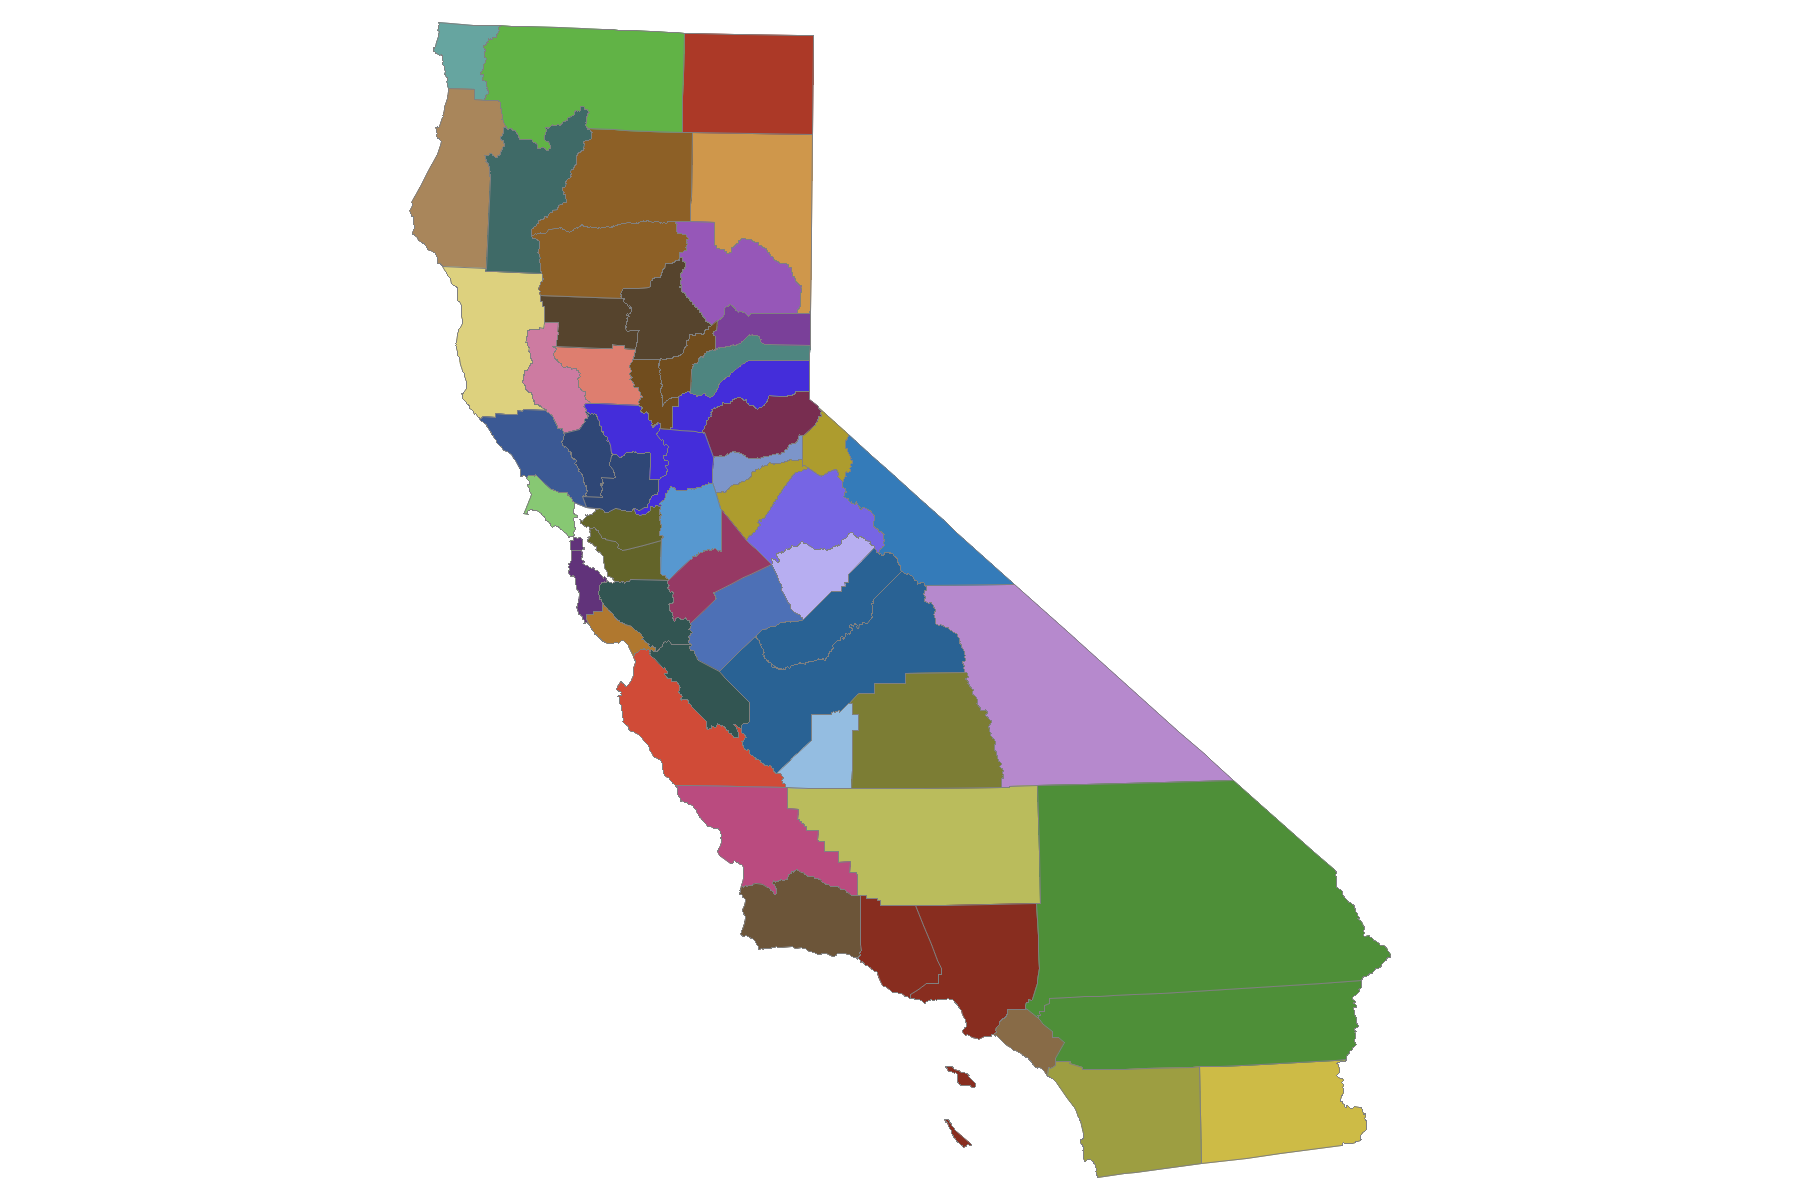
\includegraphics[scale=0.1]{./figures/insetmaps/california_clustermap_800_inset6.png} & 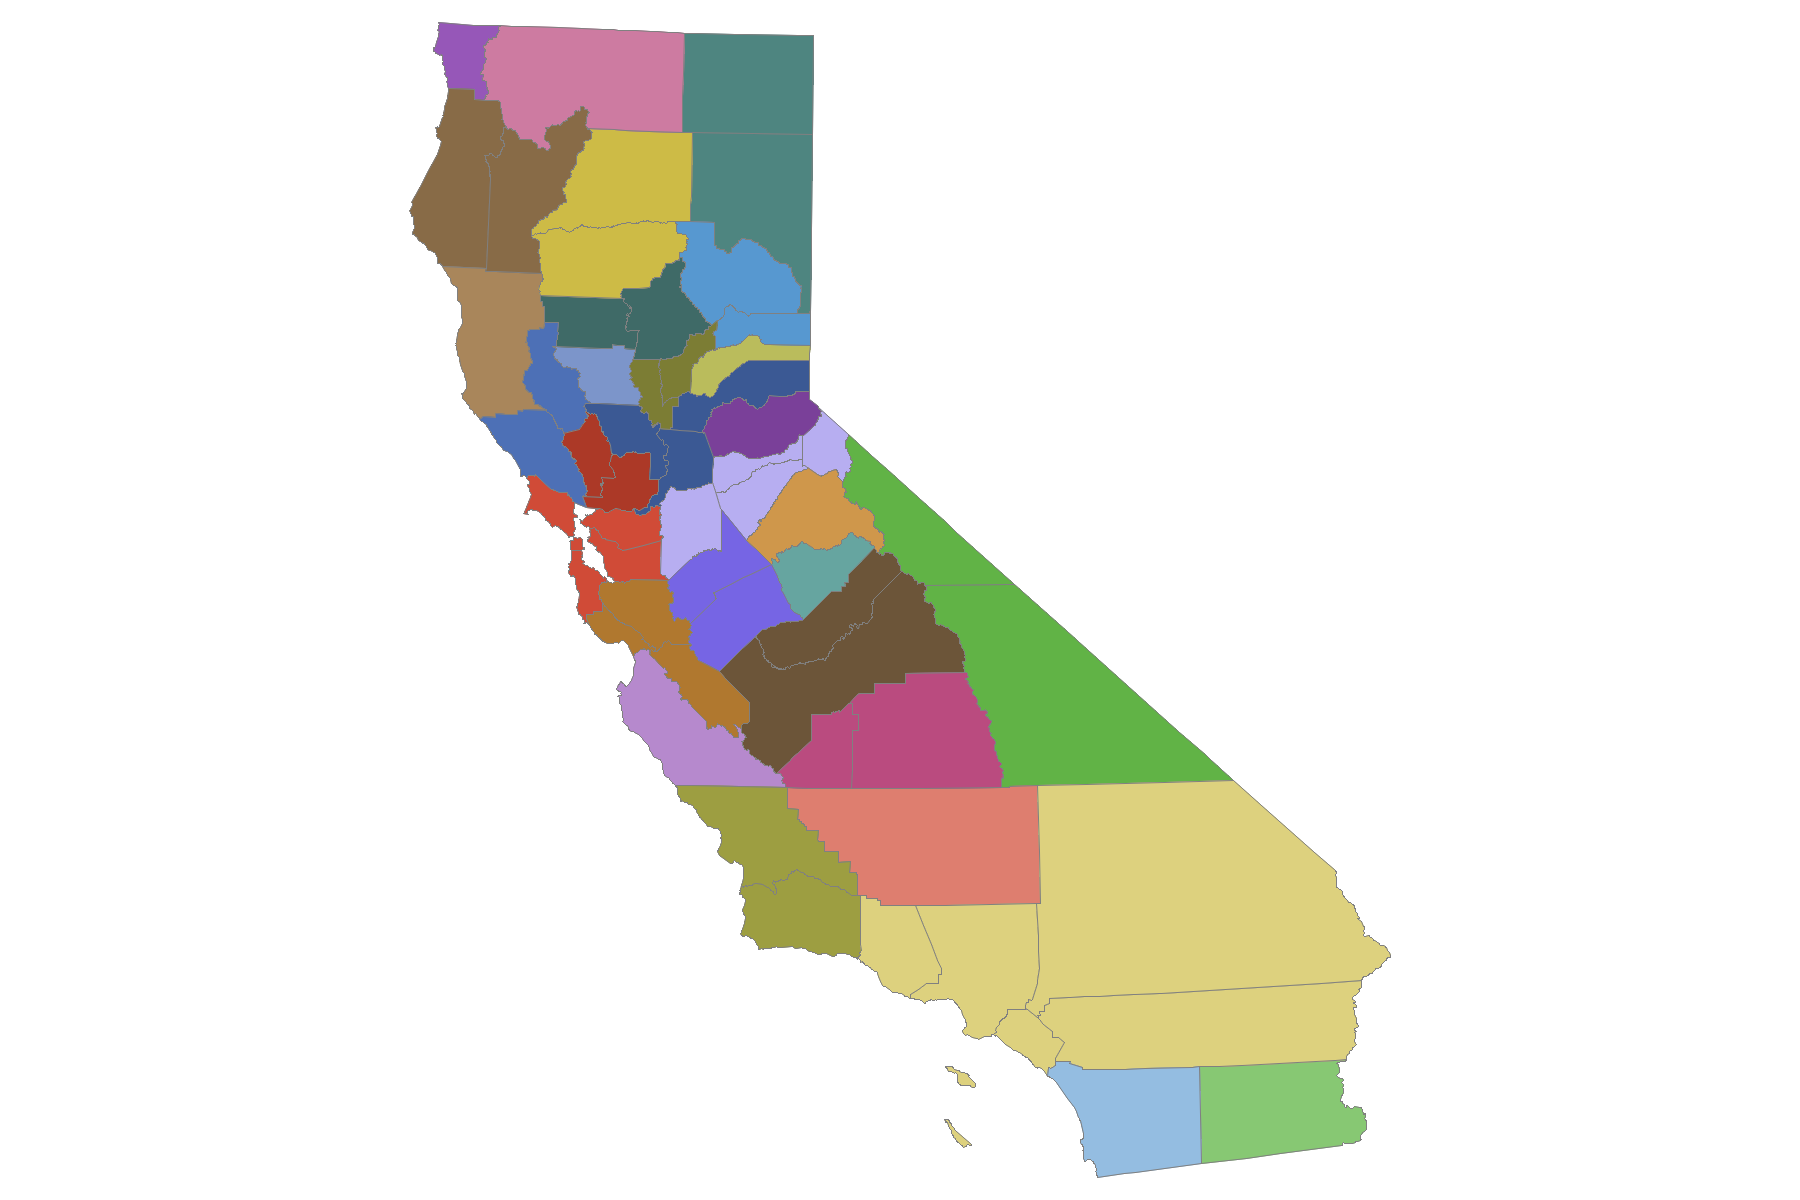
\includegraphics[scale=0.1]{./figures/insetmaps/california_clustermap_880_inset6.png} \\
Height = 0.8 & Height = 0.88 \\
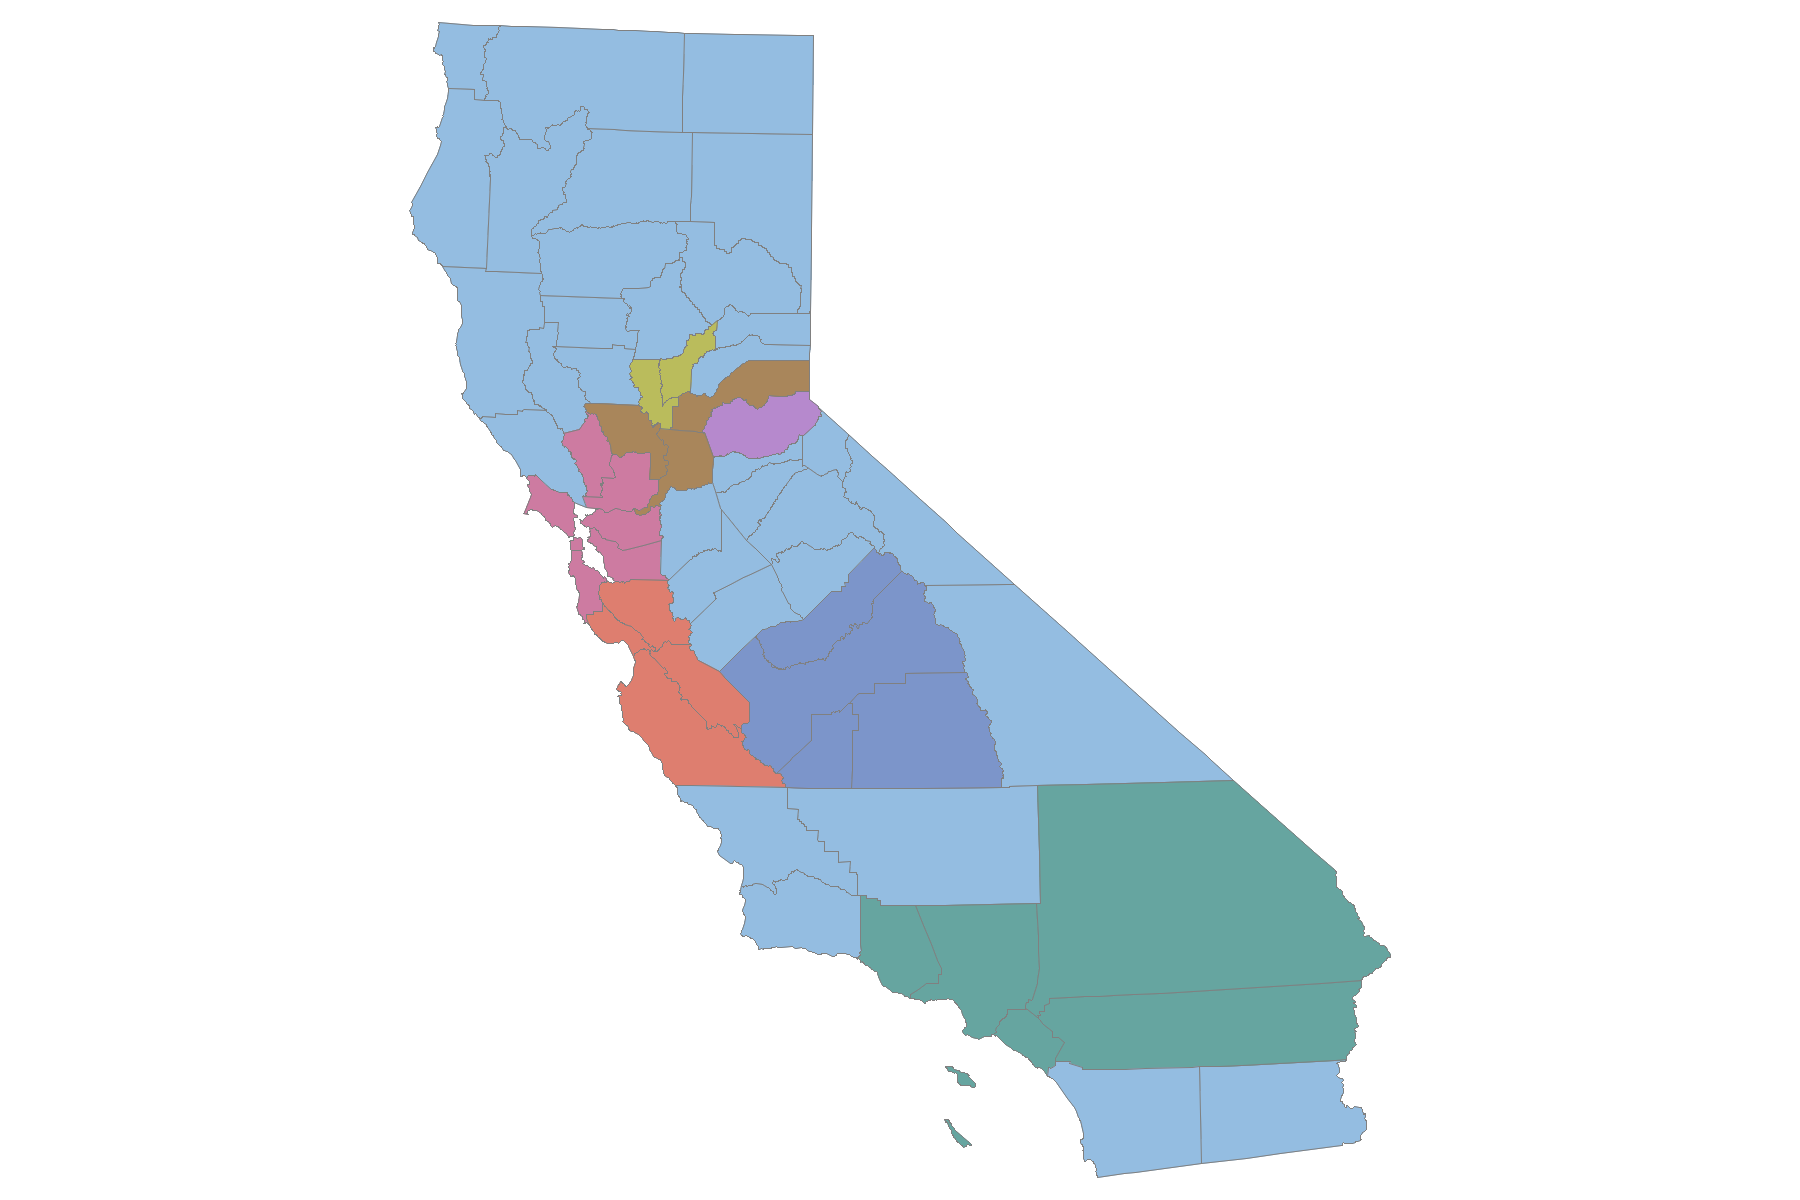
\includegraphics[scale=0.1]{./figures/insetmaps/california_clustermap_960_inset6.png} & 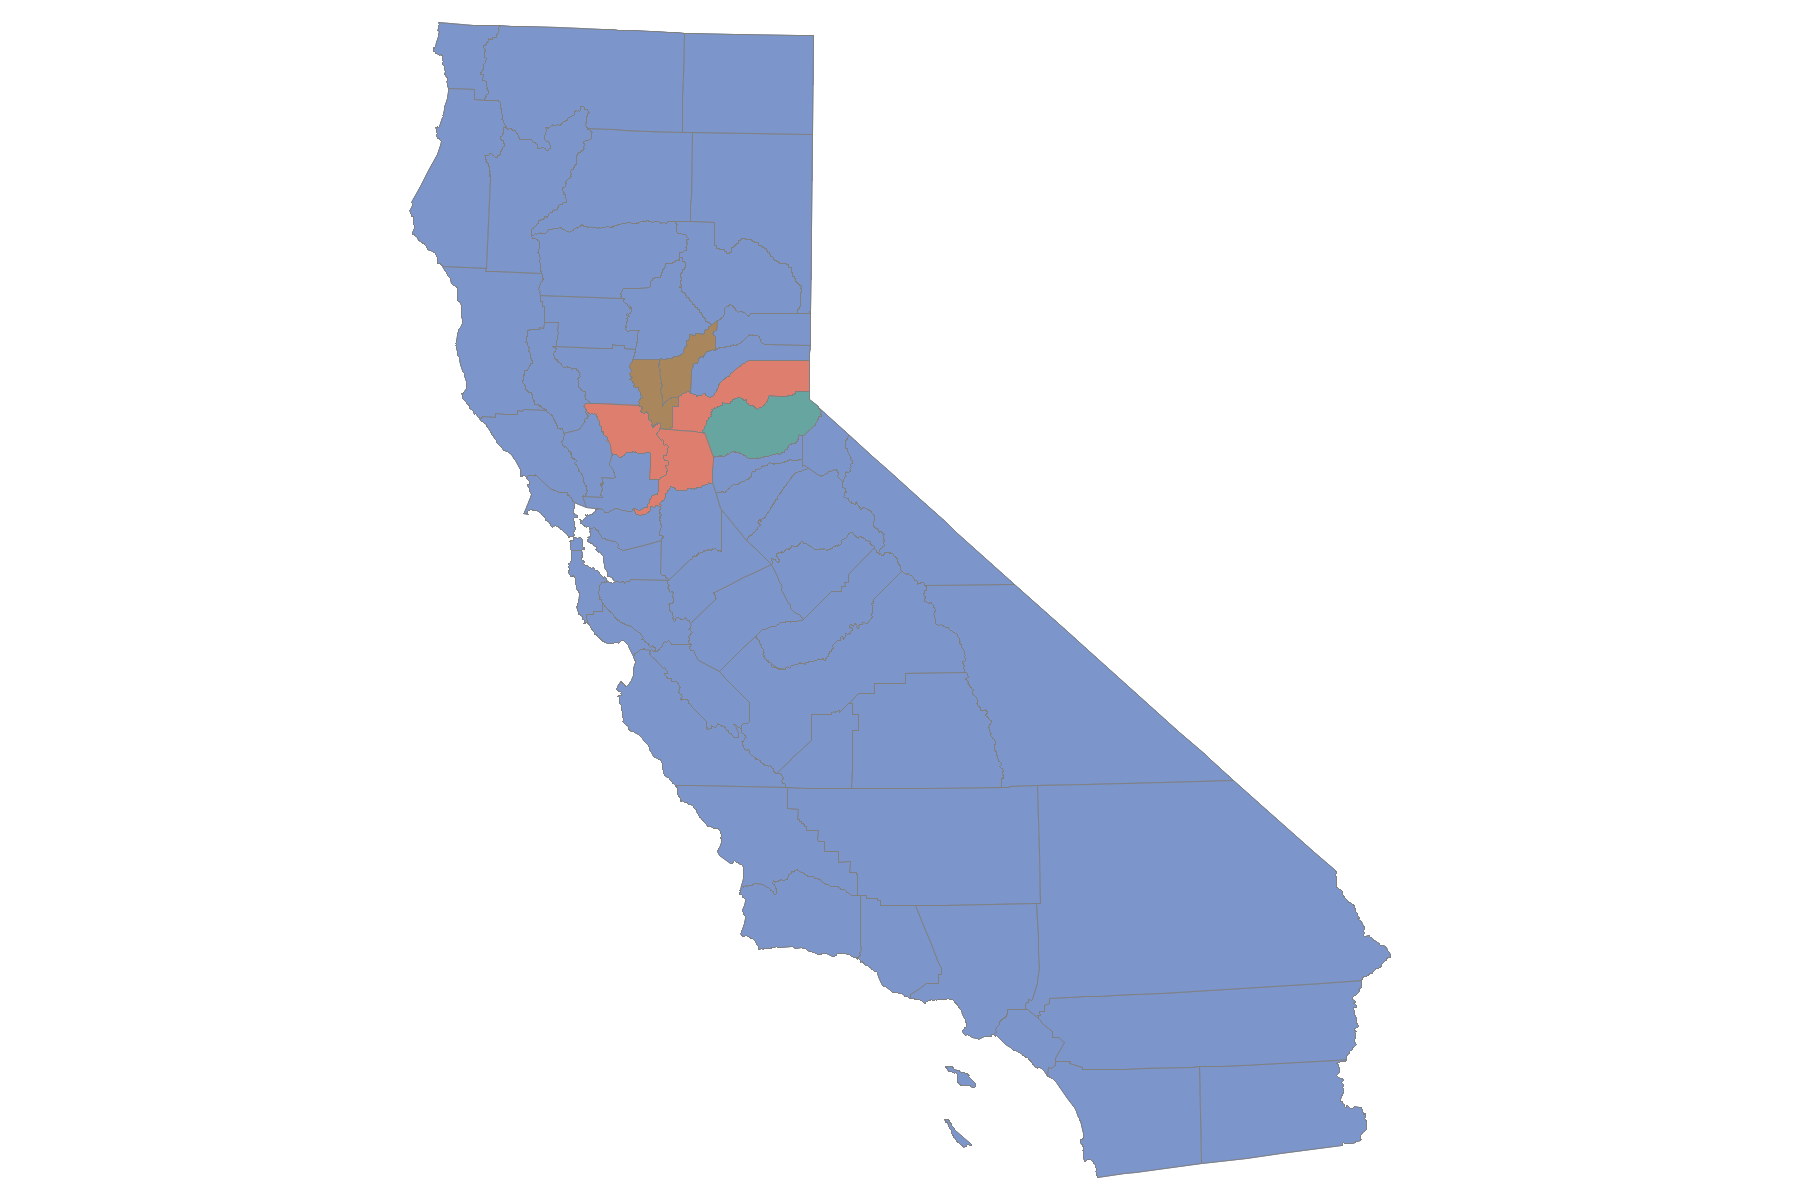
\includegraphics[scale=0.1]{./figures/insetmaps/california_clustermap_1000_inset6.png} \\
Height = 0.96 & Height = 1\\
\multicolumn{2}{p{5in}}{\footnotesize \emph{Notes:} The above graphs are generated using the methodology outlined in Section \ref{sec:method}, using 1990 Census JTW data. More detail is in the text.}
\end{tabular}
\end{figure}

\begin{table}[h]
\caption{Summary Statistics of Ratio of MOE to Flows \label{tab:moesum}}
\begin{tabular}{lcccc}
\hline\hline
& Mean & 25th Pctile & 50th Pctile & 75th Pctile \\
\hline
All counties & 1.236 & 0.845 & 1.370 & 1.600\\
Flows <100 & 1.432 & 1.148 & 1.500 & 1.636 \\
Flows 100-1000 & 0.444 & 0.301 & 0.414 & 0.549  \\
Flows 1000-10000 & 0.131 & 0.087 & 0.124 & 0.169 \\
Flows 10000+ & 0.037 & 0.024 & 0.036 & 0.049 \\
\hline\hline
\multicolumn{5}{p{4in}}{\footnotesize \emph{Notes:} Author's calculation using
2009-2013 ACS Journey-to-Work data.}
\end{tabular}
\end{table}






\end{document}
